\section{Durchführung}
\label{sec:Durchführung}
Die optischen Elemente, also die Lichtquelle, der Gegenstand, die Linsen 
und der Schirm werden auf einer optischen Bank auf Reitern befestigt.
Hier ist auf die gleiche Höhe und Neigung der Elemente zu achten.
An dieser Bank ist eine Skala integriert,
an dem die verschiedenen Abstände zueinander abgelesen werden können.
Zur Messung der Bildgrößen und Gegenstandsgrößen wird ein Lineal verwendet.
Diese Reiter ermöglichen das Verschieben dieser Elemente auf der optischen Bank.
Die Lichtquelle ist als Halogenlampe und der Gegenstand als "Perl L" realisiert.
Weiterhin werden Linsen bekannter Brennweite (hier $f=\SI{100}{\milli\meter}$ und
$f=-\SI{100}{\milli\meter}$) und eine Linse unbekannter Brennweite verwendet. \\
Die Linse unbekannter Brennweite entspricht einer mit Wasser gefüllten Linse, wobei das Wasservolumen
innerhalb dieser Linse mit Hilfe einer Spritze variiert werden kann. Aufgrund der
geänderten Krümmung erhöht sich der Brechungsindex und somit die Brennweite der Linse.
\subsection{Bestimmung der Brennweite einer Sammellinse durch Messung der Gegenstandsweite $g$ und der Bildweite $g$}
Bei der Bestimmung der Brennweite einer Sammellinse durch die Messung der Gegenstandsweite $g$ und
der Bildweite $b$ werden die Halogenlampe, die Gegenstandshalterung, die betrachtete
Linse und der Schirm
in dieser Reihenfolge auf der optischen Bank auf Reitern befestigt.
Der Gegenstand - das "Perl L" - wird an der Gegenstandshalterung angebracht.
\subsubsection{zur Verifizierung der Gleichungen}
Zu Beginn wird die Gegenstandgröße $G$ - die Größe des "Perl L"s - mit dem Lineal gemessen.
Daraufhin werden für zehn Gegenstandsweiten $g$ die Bildweiten $b$ bestimmt, bei denen auf dem
Schirm ein scharfes reelles Bild zu erkennen ist. Hierfür soll der Schirm verschoben werden.
Des Weiteren werden für die ersten fünf Messungen die Bildgrößen auf dem Schirm mit
einem Lineal bestimmt. Es werden also zehn Wertepaare $(g_{\mathrm{i}},b_{\mathrm{i}})$ und
fünf Bildgrößen notiert.
\subsubsection{Bestimmung der Brennweite einer unbekannten Sammellinse}
Die Messung der Brennweite der mit Wasser gefüllten Linse erfolgt analog zur vorherigen
Messung. Es werden allerdings nur zehn Wertepaare $(g_{\mathrm{i}},b_{\mathrm{i}})$
benötigt.\\
Hierbei ist zu beachten, dass ein konstanter Druck auf die Spritze ausgeübt wird,
damit das Wasservolumen in der Linse konstant bleibt.

\subsection{Bestimmung der Brennweite einer Sammellinse nach der Methode von Bessel für
weißes, rotes und blaues Licht}
\label{sec:bessel}
Die Anordnung der optischen Elemente für die Messung nach der Methode von Bessel ist identisch
zu der Anordnung bei der Bestimmung der Brennweite über die Messung der Gegenstandsweite und der
Bildweite.
Da die chromatische Abberration untersucht werden soll, werden für die jeweiligen
Messdurchgänge ein Rot- bzw. Blaufilter vor dem Gegenstand angebracht.
\begin{figure}
	\centering
	\begin{subfigure}[b]{0.48\textwidth}
  \centering
  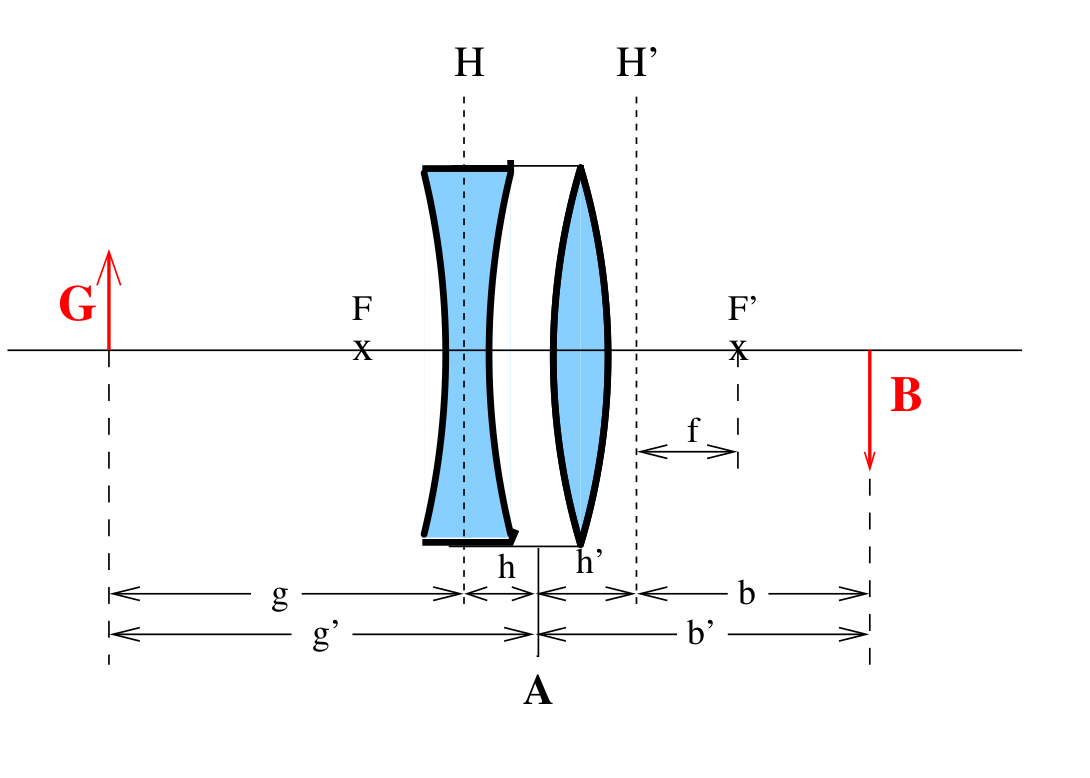
\includegraphics[width=1.0\textwidth]{Bilder/Linselol.png}
  \caption{Schematischer Aufbau des Linsensystems für die Bestimmung dessen Brennweite nach der Methode von Abbe.}
  \label{fig:lensesystemlol}
\end{subfigure}
	\begin{subfigure}[b]{0.48\textwidth}
  \centering
  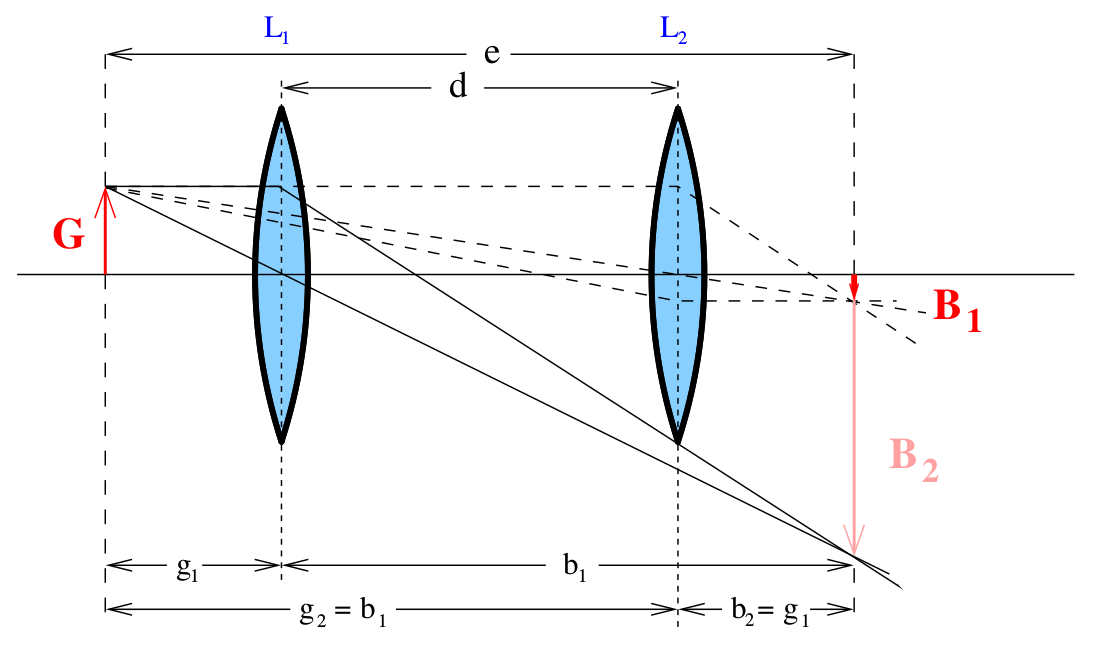
\includegraphics[width=1.0\textwidth]{Bilder/Bessel.png}
  \caption{Schematische Darstellung der beiden Linsenpositionen an denen ein scharfes Bild auf dem Schirm entsteht zur Bestimmung der Brennweite nach der Bessel-Methode.}
  \label{fig:besselmess}
\end{subfigure}
\end{figure}
Bei der Messung für die Methode nach Bessel wird wieder die Linse mit der Brennweite
$f=\SI{100}{\milli\meter}$ angebracht.
Dann wird der Abstand zwischen Gegenstand und Schirm festgehalten und die Linse solange variiert
bis beide Punkte bestimmt sind (vgl. Abbildung \ref{fig:besselmess}) , an denen ein scharfes Bild am Schirm zu sehen ist.
Für diese beiden Punkte werden jeweils die Gegenstandsweite $g_{1,2}$ und die Bildweite
$b_{1,2}$ notiert. Diese Messung soll für zehn verschiedene Abstände zwischen Gegenstand und Schirm
durchgeführt werden.\\
Die Messung wird für den bĺauen bzw. roten Filter fünfmal wiederholt.
\subsubsection{Bestimmung der Brennweite eines Linsensystems nach der Methode von Abbe}
\label{sec:abbe}
Für die Bestimmung der Brennweite eines Linsensystems wird der Aufbau aus Abbildung
\ref{fig:lensesystemlol} verwendet.
Die einzige Veränderung ist also eine zusätzliche Zerstreuungslinse mit einer Brennweite von
$f_{\mathrm{Z}} = -\SI{100}{\milli\meter}$ (Sammellinse mit $f_{\mathrm{S}}=\SI{100}{\milli\meter}$).
Für die Messung nach der Methode von Abbe wird vor der Sammellinse die Zerstreuungslinse mit
Brennweite $f_{\mathrm{Z}}=-\SI{100}{\milli\meter}$ - wie in Abschnitt \ref{sec:abbe}
beschrieben - angebracht. Der Punkt A wird als Berührungspunkt der beiden Reiter, auf denen
sich die Linsen befinden, festgelegt und die Hilfsgegenstandsweite $g'$  und Hilfsbildweite $b'$ wieder zehnmal
gemessen bis ein scharfes Bild auf dem Schirm zu erkennen ist.
